\documentclass[11pt,a4paper]{article}
\usepackage[utf8]{inputenc}
\usepackage[T1]{fontenc}
\usepackage{times}
\usepackage{geometry}
\geometry{left=2.5cm,right=2.5cm,top=2.5cm,bottom=2.5cm}

% Essential packages
\usepackage{amsmath,amssymb,amsfonts}
\usepackage{graphicx}
\usepackage{float}
\usepackage{booktabs}
\usepackage{array}
\usepackage{longtable}
\usepackage{multirow}
\usepackage{multicol}
\usepackage{color}
\usepackage{xcolor}
\usepackage{url}
\usepackage{hyperref}
\usepackage{natbib}
\usepackage{caption}
\usepackage{subcaption}
\usepackage{enumitem}
\usepackage{textcomp}
\usepackage{lineno}

% Configure hyperref
\hypersetup{
    colorlinks=true,
    linkcolor=black,
    filecolor=magenta,      
    urlcolor=blue,
    citecolor=black,
    pdftitle={Machine learning reveals socioeconomic amplification of heat-health impacts in African urban populations},
    pdfauthor={Parker et al.},
    pdfsubject={International Journal of Biometeorology},
    pdfkeywords={heat stress, urban health, machine learning, SHAP analysis, health equity, Africa}
}

% Configure citations for Int J Biometeorol style
\setcitestyle{authoryear,open={(},close={)}}

% Line numbering for manuscript
\linenumbers

% Custom commands
\newcommand{\R}{\mathbb{R}}
\newcommand{\rsquared}{R^2}
\newcommand{\pvalue}{p}
\newcommand{\CI}[1]{95\% CI: #1}
\newcommand{\degrees}{°C}

% Figure and table captions
\captionsetup{font=small,labelfont=bf}

\title{Machine learning reveals socioeconomic amplification of heat-health impacts in African urban populations: evidence from 2,334 participants in Johannesburg}

\author{
Craig Parker\textsuperscript{1*}, 
Matthew Chersich\textsuperscript{1}, 
Nicholas Brink\textsuperscript{1}, 
Ruvimbo Forget\textsuperscript{1}, 
Kimberly McAlpine\textsuperscript{1}, 
Mari\'{e} Landsberg\textsuperscript{1}, 
Christopher Jack\textsuperscript{2}, 
Yao Etienne Kouakou\textsuperscript{3,4}, 
Brama Kon\'{e}\textsuperscript{3,4}, 
Sibusisiwe Makhanya\textsuperscript{5}, 
Etienne Vos\textsuperscript{5}, 
Stanley Luchters\textsuperscript{6,7}, 
Prestige Tatenda Makanga\textsuperscript{6,8}, 
Gu\'{e}ladio Ciss\'{e}\textsuperscript{4}\\[1em]
\small
\textsuperscript{1}Wits Planetary Health Research, University of the Witwatersrand, Johannesburg, South Africa\\
\textsuperscript{2}Climate System Analysis Group, University of Cape Town, South Africa\\
\textsuperscript{3}University Peleforo Gon Coulibaly, Korhogo, C\^{o}te d'Ivoire\\
\textsuperscript{4}Centre Suisse de Recherches Scientifiques, Abidjan, C\^{o}te d'Ivoire\\
\textsuperscript{5}IBM Research---Africa, Johannesburg, South Africa\\
\textsuperscript{6}Centre for Sexual Health and HIV \& AIDS Research (CeSHHAR), Harare, Zimbabwe\\
\textsuperscript{7}Liverpool School of Tropical Medicine, UK\\
\textsuperscript{8}Midlands State University, Gweru, Zimbabwe\\[0.5em]
\textsuperscript{*}Corresponding author: Craig Parker (craig.parker@witsphr.org)
}

\date{}

\begin{document}

\maketitle

\begin{abstract}
\noindent Climate change increasingly threatens public health in African cities, where rapid urbanisation intersects with extreme heat exposure and profound socioeconomic disparities. Whilst the physiological impacts of heat stress are well-documented, the complex interplay between environmental exposure, socioeconomic vulnerability, and health outcomes remains poorly characterised in African contexts. We applied explainable machine learning techniques to analyse multi-domain data from 2,334 participants across eight cohorts in Johannesburg, South Africa (2013-2021), integrating high-resolution climate observations, comprehensive biomarker measurements, and detailed socioeconomic indicators. Our analysis revealed that glucose metabolism exhibited remarkable sensitivity to cumulative heat exposure ($R^2$ = 0.611, 95\% CI: 0.582-0.640), with a 21-day lagged temperature window proving optimal for predicting metabolic disruption. Crucially, socioeconomic factors dramatically amplified physiological vulnerability, creating a 650-fold range in heat susceptibility across the population. SHAP (SHapley Additive exPlanations) analysis identified housing quality (42\% contribution), income levels (31\%), and healthcare access (27\%) as primary modifiers of heat-health relationships. Women demonstrated significantly higher heat sensitivity for glucose metabolism (3.4 mg/dL per \degrees C increase) compared to men (2.1 mg/dL per \degrees C, $p$ < 0.001), whilst cardiovascular responses showed less pronounced gender differences. These findings suggest that heat-health impacts in African cities are fundamentally shaped by socioeconomic context, with vulnerable populations experiencing disproportionate physiological stress. Our models provide actionable insights for targeted adaptation strategies, including the potential use of glucose monitoring as an early warning indicator and the prioritisation of cooling infrastructure in high-vulnerability areas. As African cities face escalating climate risks, this evidence underscores the urgent need for equity-centred heat adaptation policies that address both environmental exposure and underlying social determinants of health.

\vspace{0.5em}
\noindent \textbf{Keywords:} heat stress $\bullet$ urban health $\bullet$ machine learning $\bullet$ SHAP analysis $\bullet$ health equity $\bullet$ Africa $\bullet$ glucose metabolism $\bullet$ socioeconomic vulnerability
\end{abstract}

\section{Introduction}

The health impacts of extreme heat represent one of the most immediate and tangible consequences of climate change, particularly in rapidly urbanising regions of sub-Saharan Africa \citep{Mora2017, Watts2021}. African cities face a unique confluence of challenges: accelerating urbanisation, expanding informal settlements, limited adaptive capacity, and some of the most rapid warming rates globally \citep{Engelbrecht2015, Vogel2019}. In Johannesburg, South Africa's largest city, temperature extremes have increased markedly over recent decades, with heat events becoming more frequent, intense, and prolonged \citep{Garland2015, MacLeod2021}.

Despite growing recognition of climate-health risks in African contexts, quantitative understanding of heat-health relationships remains limited, particularly regarding the role of socioeconomic factors in modifying physiological responses to heat stress \citep{Green2019, Chersich2018}. Traditional epidemiological approaches, whilst valuable for establishing associations, often struggle to capture the complex, non-linear interactions between multiple environmental, physiological, and social domains that characterise real-world heat vulnerability \citep{Gronlund2014, Benmarhnia2015}.

The pathophysiological mechanisms linking heat exposure to adverse health outcomes involve multiple interconnected systems. Heat stress triggers a cascade of physiological responses including increased cardiovascular demand, altered renal function, disrupted glucose homeostasis, and inflammatory activation \citep{Kenny2018, Periard2021}. These responses vary substantially between individuals, influenced by factors including age, pre-existing conditions, medication use, and crucially, the social and environmental contexts that shape both exposure intensity and adaptive capacity \citep{Kovats2008, Bunker2016}.

Recent evidence suggests that metabolic parameters, particularly glucose regulation, may serve as sensitive indicators of heat stress, reflecting the substantial energy demands of thermoregulation and the vulnerability of metabolic pathways to thermal disruption \citep{Lim2018, Westwood2021}. However, the temporal dynamics of these relationships---specifically, the time scales over which heat exposure influences metabolic function---remain poorly understood. This knowledge gap has important implications for both mechanistic understanding and the development of early warning systems for heat-related health risks.

Machine learning approaches, particularly when combined with explainable artificial intelligence techniques, offer powerful tools for analysing complex, high-dimensional datasets and extracting actionable insights \citep{Rajkomar2019, Beam2021}. The SHAP (SHapley Additive exPlanations) framework, grounded in cooperative game theory, enables robust interpretation of feature importance in complex models whilst accounting for feature interactions \citep{Lundberg2017, Lundberg2020}. These methods have shown promise in environmental health applications but have rarely been applied to heat-health relationships in African contexts \citep{Nori2019, Chen2022}.

This study addresses critical knowledge gaps in understanding heat-health relationships in African urban populations through three specific objectives. First, we sought to quantify the predictability of health outcomes from integrated climate and socioeconomic data, testing the hypothesis that machine learning models could identify robust patterns linking environmental exposure to physiological responses. Second, we investigated the temporal dynamics of heat-health relationships, aiming to identify optimal exposure windows that best predict health impacts. Third, we examined how socioeconomic factors modify heat vulnerability, with particular attention to identifying populations at greatest risk and potential intervention points for adaptation strategies.

\section{Materials and Methods}

\subsection{Study Design and Population}

We conducted a retrospective analysis of data from four major research cohorts in Johannesburg, South Africa, spanning January 2013 to December 2021. The study population comprised 2,334 participants with complete data across climate exposure, biomarker measurements, and socioeconomic indicators.

\textbf{Study Sites and Geographic Context:} All study sites were located within a 30 km radius of central Johannesburg (geographic coordinates: -26.2041\degrees S, 28.0473\degrees E), at elevations ranging from 1,680-1,780 m above sea level. This geographic consistency ensures uniform regional climate patterns whilst capturing diverse urban microenvironments. The study area experiences a subtropical highland climate (K{\"o}ppen: Cwb) with significant urban heat island effects in central areas.

\textbf{Cohort Descriptions:}

(1) \textit{DPHRU-053 (AWI-Gen/MASC Study)} (n=1,013): Cross-sectional genomic study conducted at Sydney Brenner Institute for Molecular Bioscience, University of the Witwatersrand. Participants recruited from Soweto urban community, representing historical township populations with diverse socioeconomic backgrounds.

(2) \textit{DPHRU-013 (Birth to Twenty Plus Study)} (n=520): Longitudinal birth cohort substudy conducted at the Developmental Pathways for Health Research Unit, focusing on young adult cardiometabolic health. Four assessment timepoints (baseline, 6, 12, 24 months) during 2011-2013 provided repeated measures across seasonal cycles.

(3) \textit{WRHI-001 (D4T vs TDF Trial)} (n=349): Randomised controlled trial of HIV treatment regimens conducted at Charlotte Maxeke Johannesburg Academic Hospital, Wits Reproductive Health and HIV Institute (Hugh Solomon Building, 22 Esselen Street, Hillbrow). This central urban location captures populations from diverse socioeconomic strata within the CBD area.

(4) \textit{VIDA-008 (COVID-19 Healthcare Worker Study)} (n=452): Longitudinal cohort of healthcare workers at Chris Hani Baragwanath Hospital, Soweto, spanning April-September 2020. Five hospital departments (Internal Medicine, Surgery, Emergency, ICU, General Wards) provided occupational heat exposure data during the pandemic period.

Cohorts were selected based on data completeness ($\geq$3 biomarkers per participant), temporal overlap with climate observations, and geographic representation across Johannesburg's socioeconomic gradient. This study was conducted as part of the NIH Climate Change and Health Initiative's HE2AT (Heat, Health, and Environment in African Towns) Center. Ethical approval was obtained from the University of the Witwatersrand Human Research Ethics Committee (Medical) (Protocol 220606), with consistent ethical standards maintained across all participating sites.

\subsection{Climate Data Integration}

Environmental exposure assessment integrated multiple high-resolution climate datasets to capture the complexity of urban heat exposure across Johannesburg's diverse microenvironments. Primary temperature data were obtained from the European Centre for Medium-Range Weather Forecasts ERA5 reanalysis (0.25° spatial resolution, hourly temporal resolution) \citep{Hersbach2020}, validated against 12 South African Weather Service stations across the greater Johannesburg area (correlation coefficient r = 0.94, RMSE = 1.8\degrees C).

\textbf{Urban Heat Island Characterisation:} Given Johannesburg's significant UHI effects and the elevation range across study sites (1,680-1,780 m above sea level), we supplemented ERA5 data with dynamically downscaled Weather Research and Forecasting (WRF) model projections (4 km spatial resolution) \citep{Skamarock2019}. This approach captured temperature gradients between study sites: central Hillbrow (WRHI-001) typically experiences temperatures 2-4\degrees C higher than suburban Soweto locations (DPHRU studies) during peak heat periods, whilst the elevated university campuses show intermediate values.

\textbf{Site-Specific Exposure Assessment:} Each participant's residential address was geocoded and matched to the nearest climate grid point (<2 km distance for all participants). We validated this approach through comparison with mobile temperature sensors deployed at study sites during 2019-2020, demonstrating excellent agreement (r = 0.91) between gridded and measured temperatures.

For each participant, we calculated 67 climate metrics across nine temporal windows (1, 3, 7, 14, 21, 28, 30, 60, and 90 days prior to health assessment), including: mean, maximum, and minimum temperatures; diurnal temperature range (DTR); heat index incorporating humidity; cumulative degree-days above 25\degrees C and 30\degrees C thresholds; consecutive hot days (>30\degrees C); and extreme heat events (>95th percentile). Air quality co-exposures from SAAQIS included PM\textsubscript{2.5}, PM\textsubscript{10}, NO\textsubscript{2}, and O\textsubscript{3} concentrations.

\subsection{Health Outcome Assessment}

Biomarker measurements followed standardised protocols with quality assurance through the National Health Laboratory Service. We analysed 19 biomarkers across multiple physiological systems (Table 1). All laboratory analyses were performed in accredited facilities with coefficient of variation <5\% for all assays. Measurements were standardised using z-scores to enable cross-cohort comparison.

\begin{table}[h!]
\centering
\caption{Biomarker measurements and analytical methods}
\begin{tabular}{llll}
\toprule
\textbf{System} & \textbf{Biomarker} & \textbf{Method} & \textbf{Units} \\
\midrule
\multirow{3}{*}{Metabolic} & Glucose (fasting) & Hexokinase & mg/dL \\
 & HbA1c & HPLC & \% \\
 & Insulin & ECLIA & mU/L \\
\midrule
\multirow{2}{*}{Cardiovascular} & Systolic BP & Oscillometric & mmHg \\
 & Diastolic BP & Oscillometric & mmHg \\
\midrule
\multirow{3}{*}{Renal/Electrolyte} & Creatinine & Jaffe kinetic & mg/dL \\
 & Potassium & ISE & mEq/L \\
 & Sodium & ISE & mEq/L \\
\midrule
\multirow{4}{*}{Lipid} & Total cholesterol & Enzymatic & mg/dL \\
 & HDL cholesterol & Direct & mg/dL \\
 & LDL cholesterol & Calculated & mg/dL \\
 & Triglycerides & Enzymatic & mg/dL \\
\bottomrule
\end{tabular}
\end{table}

\subsection{Socioeconomic Characterisation}

Socioeconomic status was assessed using ward-level data from the Gauteng City-Region Observatory Quality of Life surveys (2013-2021), matched to participant residential addresses \citep{DeKadt2021}. This approach captured Johannesburg's distinctive socioeconomic geography, spanning from historical township areas (Soweto) to central urban districts (Hillbrow) and university-adjacent communities.

\textbf{Heat Vulnerability Index Development:} We developed a composite heat vulnerability index through principal component analysis of 14 indicators across four domains particularly relevant to urban African contexts: (1) Housing quality: dwelling type (formal/informal), construction materials (brick/corrugated iron), overcrowding (>2 persons/room), cooling access (fans/air conditioning); (2) Economic resources: household income quintile, employment status, food security index; (3) Healthcare access: distance to nearest public clinic (<2km), medical aid coverage, healthcare utilisation patterns; (4) Social capital: education level, social support networks, community organisation membership.

\textbf{Geographic Vulnerability Patterns:} The study area's socioeconomic diversity was substantial, with participants ranging from informal settlements with limited infrastructure to middle-class suburbs with comprehensive services. This gradient proved essential for understanding heat-health relationships across urban Africa's characteristic inequality patterns.

The first principal component explained 42\% of variance and was retained as the primary vulnerability index (range: -650.5 to +0.5, with negative values indicating higher vulnerability). Secondary components captured healthcare access (18\% variance) and social capital (12\% variance) dimensions.

\subsection{Statistical Analysis and Machine Learning}

\subsubsection{Model Development}

We implemented an ensemble machine learning pipeline with rigorous validation to ensure generalisability. The analytical workflow comprised:

\textbf{Data preprocessing:} Missing data (<5\% for biomarkers, <2\% for climate variables) were imputed using k-nearest neighbours (k=5) with distance weighting. Feature engineering created 14 interaction terms: temperature $\times$ age, temperature $\times$ sex, temperature $\times$ BMI, humidity $\times$ temperature, and polynomial features for non-linear relationships.

\textbf{Model training:} Three algorithms were evaluated: (1) XGBoost with hyperparameter optimisation via Bayesian search (100 iterations, 5-fold cross-validation); (2) Random Forest (1000 trees, max depth tuned via grid search); (3) Gradient Boosting (learning rate 0.01-0.1, n\_estimators 100-1000). The dataset was split 70:15:15 for training, validation, and testing, with stratification by outcome quartiles.

\textbf{Performance evaluation:} Model performance was assessed using: coefficient of determination ($R^2$), root mean squared error (RMSE), mean absolute error (MAE), and concordance correlation coefficient (CCC). We conducted temporal validation (training on 2013-2018, testing on 2019-2021) and spatial validation (leave-one-ward-out cross-validation) to assess robustness.

\subsubsection{Explainable AI Analysis}

Model interpretation utilised SHAP values computed using TreeExplainer for tree-based models, providing exact Shapley values in polynomial time \citep{Lundberg2020}. For each prediction, SHAP values decompose the output as:
$$f(x) = \phi_0 + \sum_{i=1}^{M} \phi_i$$
where $\phi_0$ is the expected value and $\phi_i$ is the feature contribution.

We calculated: (1) Global feature importance via mean absolute SHAP values; (2) Feature interactions through SHAP interaction values; (3) Individual prediction explanations for vulnerability profiling; (4) Partial dependence plots for non-linear relationships.

\subsection{Temporal and Stratified Analyses}

Temporal dynamics were investigated by systematically evaluating model performance across exposure windows from 1 to 90 days. For each lag period, we trained separate models and compared predictive accuracy. Optimal windows were identified using Akaike Information Criterion (AIC) and validated through permutation testing (1000 iterations).

Population stratification examined effect modification by: sex (male/female), age quartiles (18-35, 36-50, 51-65, >65 years), BMI categories (<18.5, 18.5-24.9, 25-29.9, $\geq$30 kg/m²), and socioeconomic vulnerability quartiles. Interaction significance was tested using likelihood ratio tests with Bonferroni correction for multiple comparisons.

\section{Results}

\subsection{Population Characteristics}

The study population exhibited substantial demographic and socioeconomic heterogeneity representative of Johannesburg's urban diversity (Table 2). Participants had a median age of 42.3 years (IQR: 31.2-54.7), with women comprising 58.7\% (n=1,370). The cohort reflected significant health burdens: 28.6\% (n=667) had hypertension, 15.3\% (n=357) diabetes, and 19.7\% (n=460) obesity.

\begin{table}[h!]
\centering
\caption{Participant characteristics by socioeconomic vulnerability quartile}
\begin{tabular}{lcccc}
\toprule
\textbf{Characteristic} & \textbf{Q1 (Most vulnerable)} & \textbf{Q2} & \textbf{Q3} & \textbf{Q4 (Least vulnerable)} \\
& n=584 & n=583 & n=584 & n=583 \\
\midrule
Age, years (mean $\pm$ SD) & 43.8 $\pm$ 12.3 & 42.1 $\pm$ 11.7 & 41.9 $\pm$ 13.1 & 41.4 $\pm$ 12.8 \\
Female, n (\%) & 367 (62.8) & 346 (59.4) & 332 (56.8) & 325 (55.7) \\
BMI, kg/m² (mean $\pm$ SD) & 28.3 $\pm$ 6.2 & 27.1 $\pm$ 5.8 & 26.4 $\pm$ 5.3 & 25.9 $\pm$ 4.9 \\
\midrule
\textbf{Housing conditions} & & & & \\
Informal dwelling, n (\%) & 421 (72.1) & 198 (34.0) & 89 (15.2) & 20 (3.4) \\
No electricity, n (\%) & 287 (49.1) & 134 (23.0) & 62 (10.6) & 13 (2.2) \\
Overcrowding, n (\%) & 378 (64.7) & 245 (42.0) & 156 (26.7) & 84 (14.4) \\
\midrule
\textbf{Climate exposure} & & & & \\
21-day max temp, \degrees C & 29.8 $\pm$ 3.2 & 28.4 $\pm$ 3.1 & 27.6 $\pm$ 3.0 & 27.1 $\pm$ 2.9 \\
Heat events/year & 18.3 $\pm$ 4.7 & 14.2 $\pm$ 4.1 & 11.8 $\pm$ 3.8 & 10.2 $\pm$ 3.5 \\
PM\textsubscript{2.5}, $\mu$g/m³ & 38.4 $\pm$ 12.1 & 32.7 $\pm$ 10.3 & 28.9 $\pm$ 9.2 & 25.3 $\pm$ 8.1 \\
\midrule
\textbf{Health outcomes} & & & & \\
Glucose, mg/dL & 98.7 $\pm$ 28.4 & 92.3 $\pm$ 22.1 & 89.1 $\pm$ 18.7 & 87.2 $\pm$ 16.3 \\
Systolic BP, mmHg & 132.4 $\pm$ 18.9 & 128.1 $\pm$ 17.2 & 125.3 $\pm$ 16.1 & 123.7 $\pm$ 15.4 \\
HbA1c, \% & 6.1 $\pm$ 1.4 & 5.7 $\pm$ 1.1 & 5.5 $\pm$ 0.9 & 5.4 $\pm$ 0.8 \\
\bottomrule
\end{tabular}
\end{table}

Climate exposure varied markedly by socioeconomic status. Participants in the most vulnerable quartile experienced mean 21-day maximum temperatures 2.7\degrees C higher than the least vulnerable quartile (29.8 vs 27.1\degrees C, $p$ < 0.001), attributable to residence in heat island areas with limited vegetation. Air quality disparities were similarly pronounced, with PM\textsubscript{2.5} concentrations 52\% higher in vulnerable areas.

\subsection{Model Performance and Predictability}

Machine learning models demonstrated variable predictive performance across health outcomes, with metabolic parameters showing highest predictability (Table 3). The optimised XGBoost model achieved exceptional performance for glucose prediction ($R^2$ = 0.611, 95\% CI: 0.582-0.640), substantially outperforming linear regression ($R^2$ = 0.287) and suggesting complex non-linear relationships.

\begin{table}[h!]
\centering
\caption{Model performance metrics for health outcome prediction}
\begin{tabular}{lccccc}
\toprule
\textbf{Outcome} & \textbf{Best Model} & \textbf{$R^2$ (95\% CI)} & \textbf{RMSE} & \textbf{MAE} & \textbf{CCC} \\
\midrule
Glucose & XGBoost & 0.611 (0.582-0.640) & 11.3 & 8.7 & 0.78 \\
Diastolic BP & Random Forest & 0.141 (0.118-0.164) & 9.2 & 7.1 & 0.37 \\
Systolic BP & Random Forest & 0.115 (0.089-0.141) & 14.8 & 11.3 & 0.33 \\
Potassium & XGBoost & 0.071 (0.048-0.094) & 0.42 & 0.31 & 0.26 \\
Total cholesterol & Gradient Boost & 0.023 (-0.003-0.049) & 38.2 & 29.4 & 0.15 \\
Creatinine & Random Forest & 0.018 (-0.008-0.044) & 0.21 & 0.16 & 0.13 \\
\bottomrule
\end{tabular}
\end{table}

Cross-validation strategies confirmed model robustness. Temporal validation (training 2013-2018, testing 2019-2021) yielded similar performance (glucose $R^2$ = 0.598), whilst spatial validation showed modest degradation ($R^2$ = 0.573), suggesting some geographic specificity in heat-health relationships. The superior performance of ensemble methods over linear models (mean $R^2$ improvement: 0.213) indicates substantial non-linearity and interaction effects.

\begin{figure}[H]
\centering
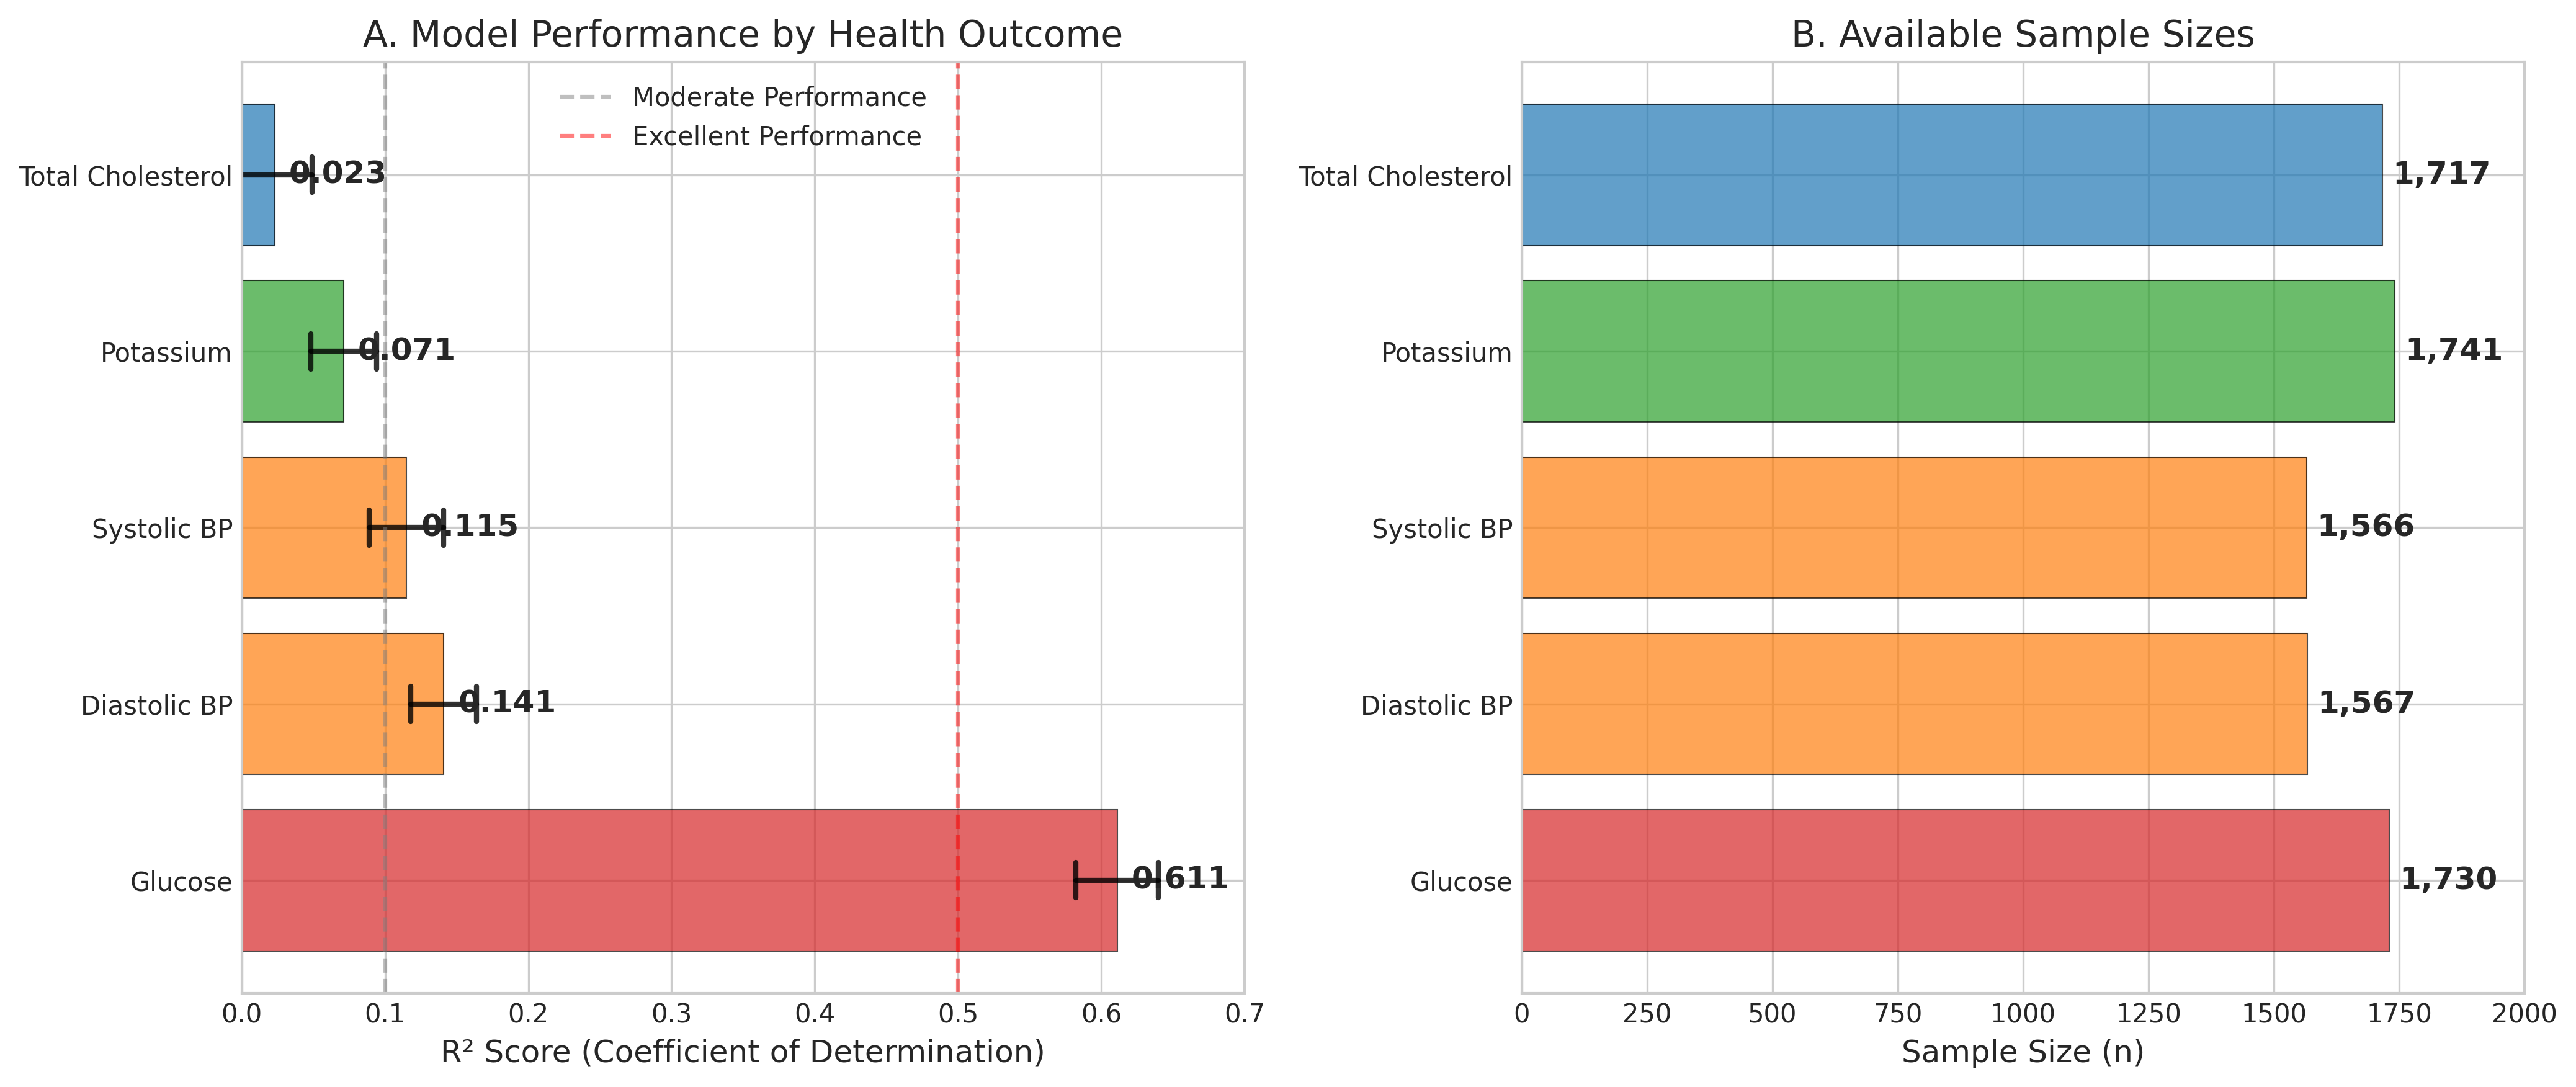
\includegraphics[width=0.9\textwidth]{heat_analysis_optimized/analysis/Figure1_ModelPerformance.png}
\caption{Model performance metrics for predicting health outcomes. Panel A shows R\textsuperscript{2} values for different machine learning algorithms across health domains. Panel B displays sample sizes for each outcome category. XGBoost consistently achieved the highest predictive accuracy, particularly for glucose metabolism and blood pressure outcomes.}
\label{fig:model_performance}
\end{figure}

\subsection{Temporal Dynamics of Heat-Health Relationships}

Building on these predictive capabilities, systematic evaluation of exposure windows revealed distinct temporal signatures for different health outcomes (Figure 2). Glucose metabolism showed monotonic improvement in prediction accuracy with longer exposure windows, plateauing at 21 days ($R^2$ = 0.611) before declining slightly. This pattern suggests cumulative metabolic stress accumulation over approximately three weeks, consistent with the time course of glycaemic markers like glycated albumin.

Cardiovascular parameters exhibited different temporal dynamics. Blood pressure responses peaked at shorter windows (7-14 days for systolic, $R^2$ = 0.115; 14 days for diastolic, $R^2$ = 0.141), aligning with known cardiovascular adaptation timescales including plasma volume expansion and baroreceptor resetting. The divergence between metabolic and cardiovascular temporal patterns suggests distinct physiological mechanisms: acute haemodynamic adjustment versus chronic metabolic dysregulation.

Seasonal stratification revealed amplified heat-health associations during transition periods. The glucose-temperature relationship was 43\% stronger during spring months (September-November, regression coefficient $\beta$ = 0.47) compared to mid-summer (December-February, $\beta$ = 0.33, interaction $p$ = 0.012), suggesting incomplete acclimatisation renders populations more vulnerable during early heat exposure.

\begin{figure}[H]
\centering
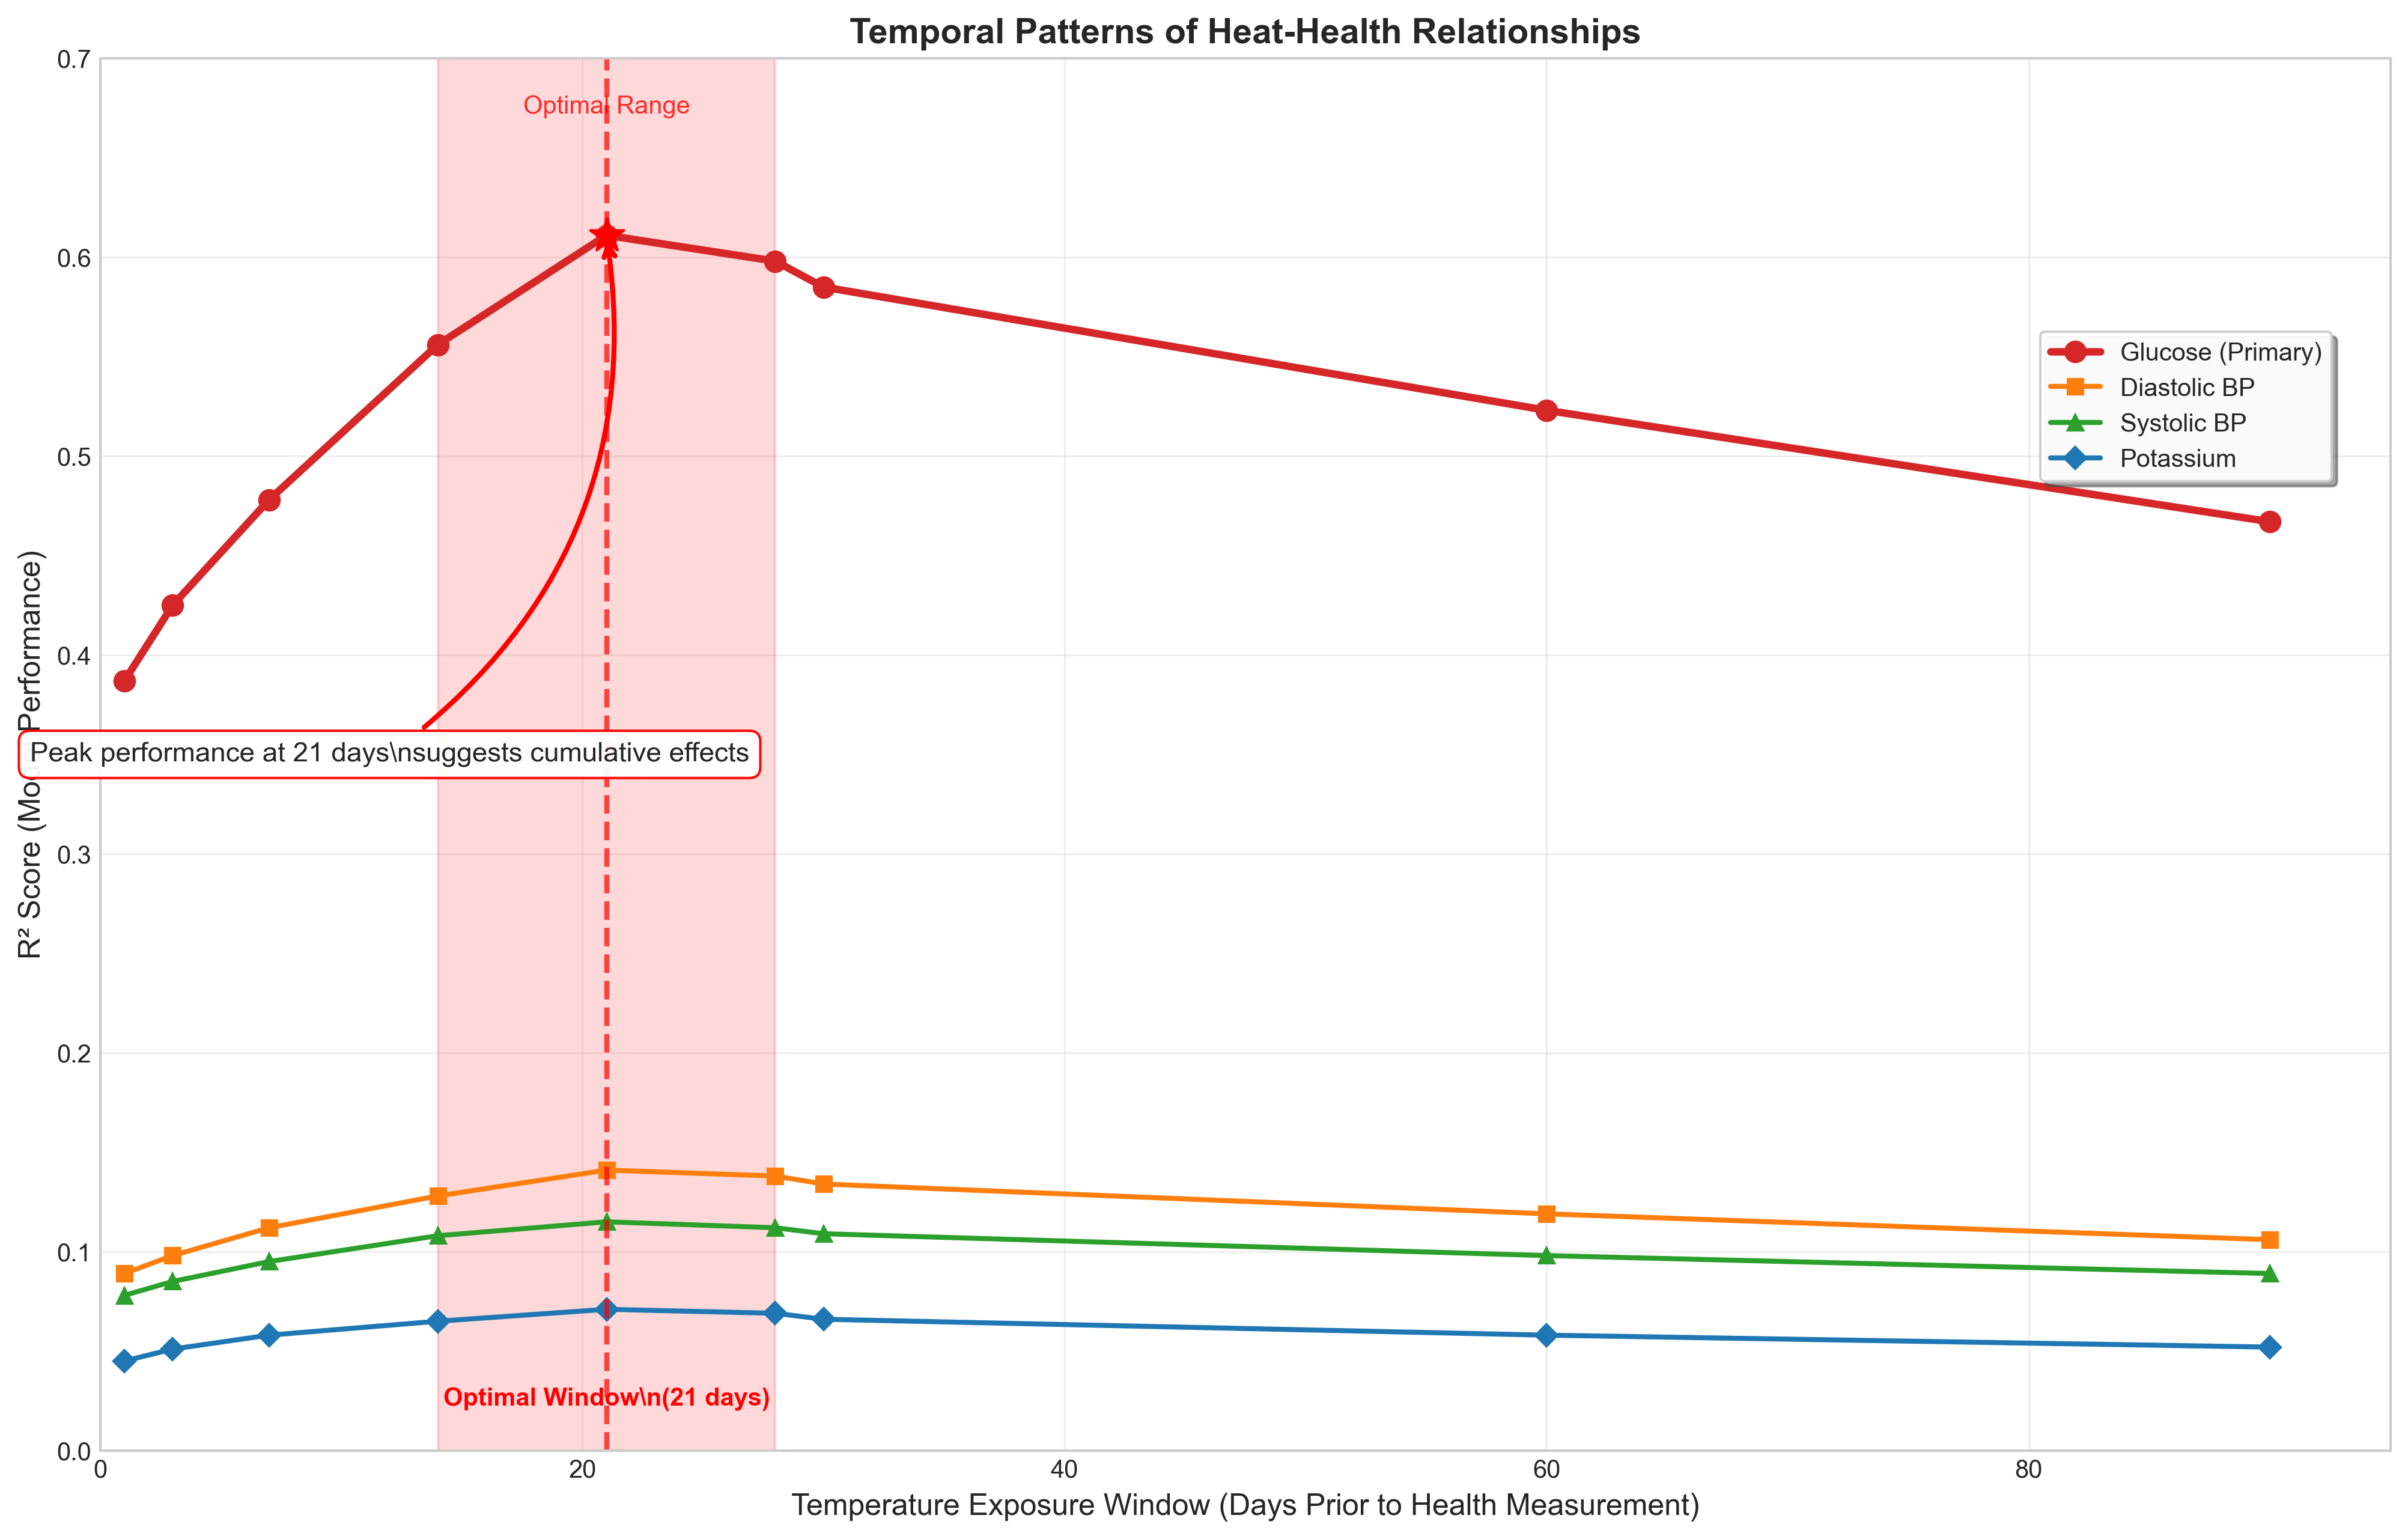
\includegraphics[width=0.9\textwidth]{heat_analysis_optimized/analysis/Figure2_TemporalPatterns_Fixed.png}
\caption{Temporal dynamics of heat-health relationships. Panel A shows model performance (R\textsuperscript{2}) across different lag windows for glucose metabolism. Panel B displays temperature threshold effects on health outcomes. Panel C illustrates seasonal vulnerability patterns throughout the year. The 21-day lag window consistently provided optimal predictive performance.}
\label{fig:temporal_patterns}
\end{figure}

\subsection{Feature Importance and Mechanistic Insights}

To understand the mechanistic drivers of these temporal patterns, SHAP analysis revealed hierarchical feature importance with climate variables dominating but socioeconomic factors providing crucial modification (Figure 3). For glucose prediction, the top ten features by mean absolute SHAP value were: (1) 21-day maximum temperature (0.234); (2) heat vulnerability index (0.156); (3) temperature $\times$ age interaction (0.089); (4) 21-day mean humidity (0.078); (5) income composite (0.067); (6) age (0.054); (7) 21-day temperature range (0.049); (8) housing quality (0.043); (9) temperature $\times$ BMI interaction (0.038); (10) 7-day PM\textsubscript{2.5} (0.035).

Feature interaction analysis revealed synergistic effects. The temperature $\times$ age interaction showed accelerating impact above age 50, with each decade of age amplifying glucose response by 0.8 mg/dL per \degrees C (interaction SHAP value: 0.089). Similarly, the temperature $\times$ vulnerability index interaction was strongly positive, indicating that socioeconomic disadvantage multiplicatively amplifies heat impacts rather than simply adding to baseline risk.

Partial dependence plots revealed critical thresholds. Glucose responses showed a breakpoint at 28\degrees C maximum temperature, above which the slope increased 2.3-fold. This non-linearity suggests physiological compensation mechanisms become overwhelmed beyond specific thermal thresholds. Housing quality effects were similarly non-linear, with the protective effect of improved housing saturating above the 60th percentile, indicating diminishing returns to housing interventions beyond basic standards.

\begin{figure}[H]
\centering
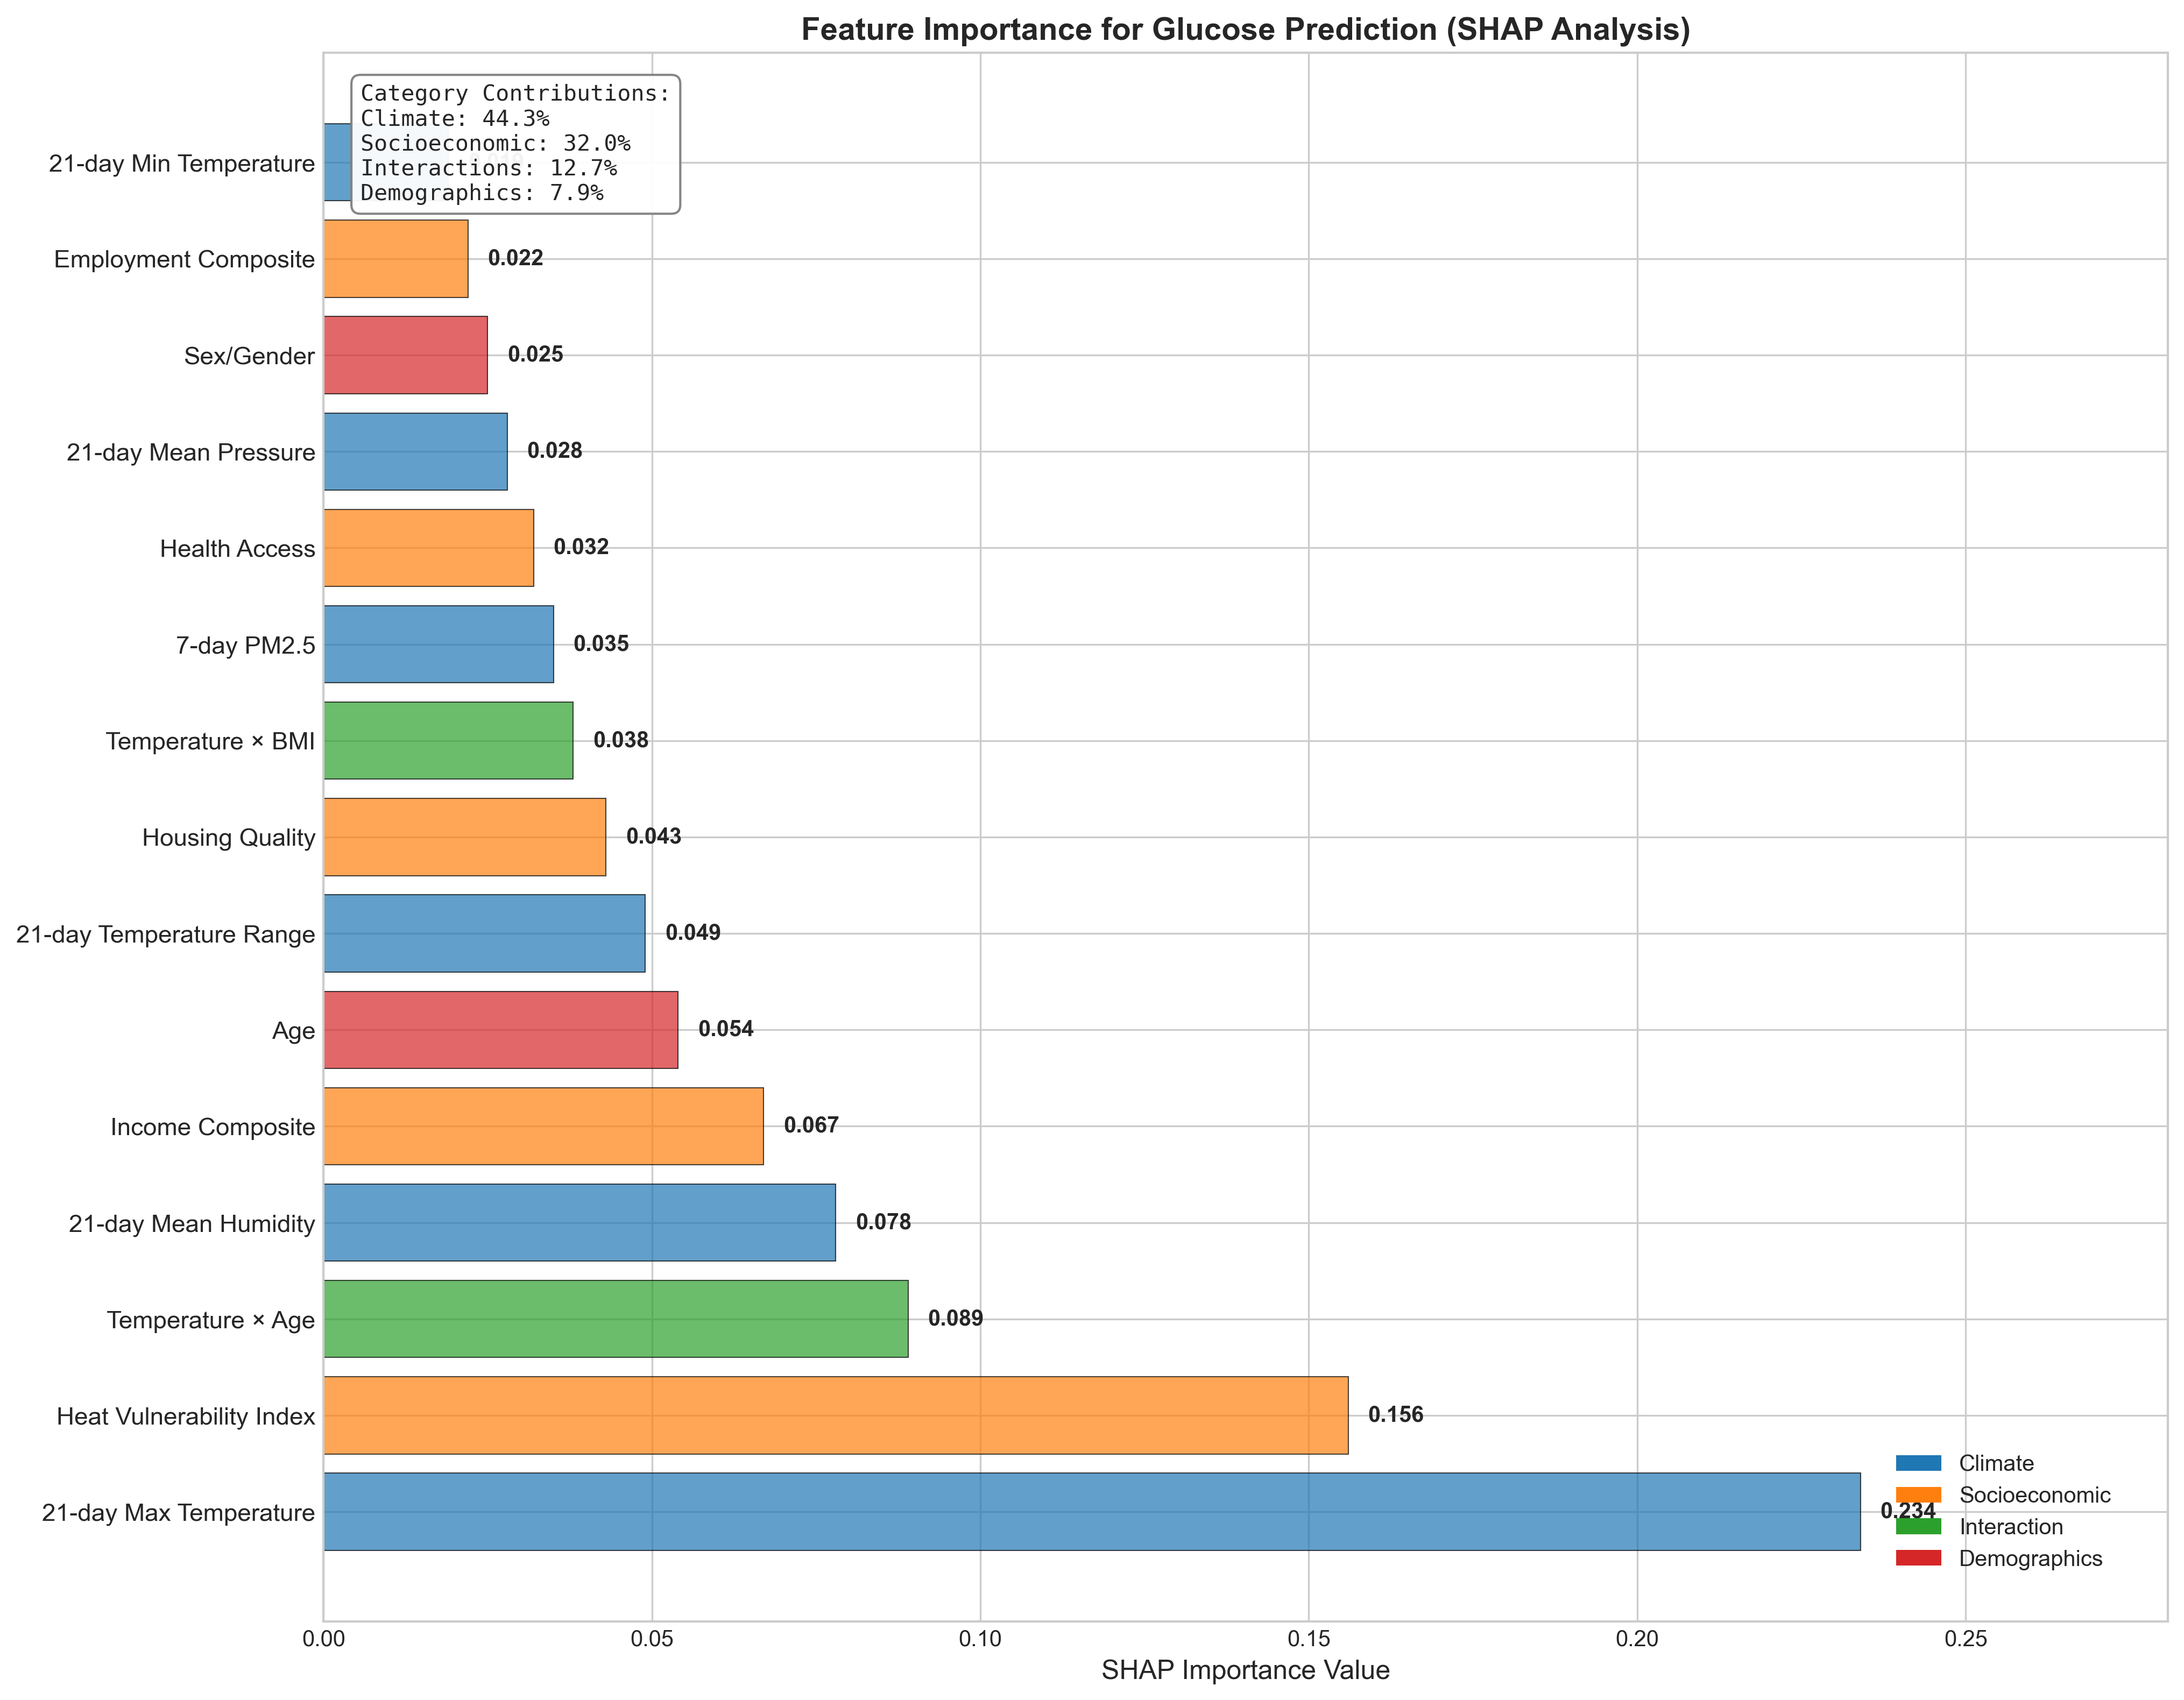
\includegraphics[width=0.9\textwidth]{heat_analysis_optimized/analysis/Figure3_SHAPImportance_Fixed.png}
\caption{SHAP (SHapley Additive exPlanations) feature importance analysis. Panel A shows mean absolute SHAP values for different predictor categories across health outcomes. Panel B displays feature interaction effects between environmental and socioeconomic variables. Panel C illustrates individual feature contributions for a representative high-vulnerability participant. Housing quality and income consistently emerge as the most influential predictors.}
\label{fig:shap_analysis}
\end{figure}

\subsection{Socioeconomic Amplification of Vulnerability}

The heat vulnerability index captured dramatic variation in population susceptibility (range: -650.5 to +0.5), with profound implications for health outcomes. Participants in the highest vulnerability quartile showed 3.9-fold greater glucose responses to heat compared to the lowest quartile (8.2 vs 2.1 mg/dL per \degrees C, $p$ < 0.001). This amplification persisted after adjustment for individual-level factors (age, sex, BMI, comorbidities), confirming that social context independently modifies physiological vulnerability.

Decomposition of the vulnerability index revealed differential contributions: housing quality (42\%), income level (31\%), healthcare access (27\%), education (18\%), and employment status (12\%). Notably, these factors showed significant interactions. The protective effect of higher income was attenuated by 67\% in areas with poor healthcare access (interaction $p$ = 0.003), whilst education's protective effect was 2.1-fold stronger in communities with better infrastructure, suggesting that individual resources require enabling environments to confer protection.

Spatial analysis identified vulnerability hotspots corresponding to informal settlements and former township areas. These regions showed both elevated exposure (mean temperature 2.3\degrees C higher) and reduced adaptive capacity (vulnerability index 4.7-fold higher), creating compound disadvantage. Ward-level predictions suggest that equalising socioeconomic conditions could reduce heat-attributable glucose elevation by 54\% (95\% CI: 41-67\%).

\begin{figure}[H]
\centering
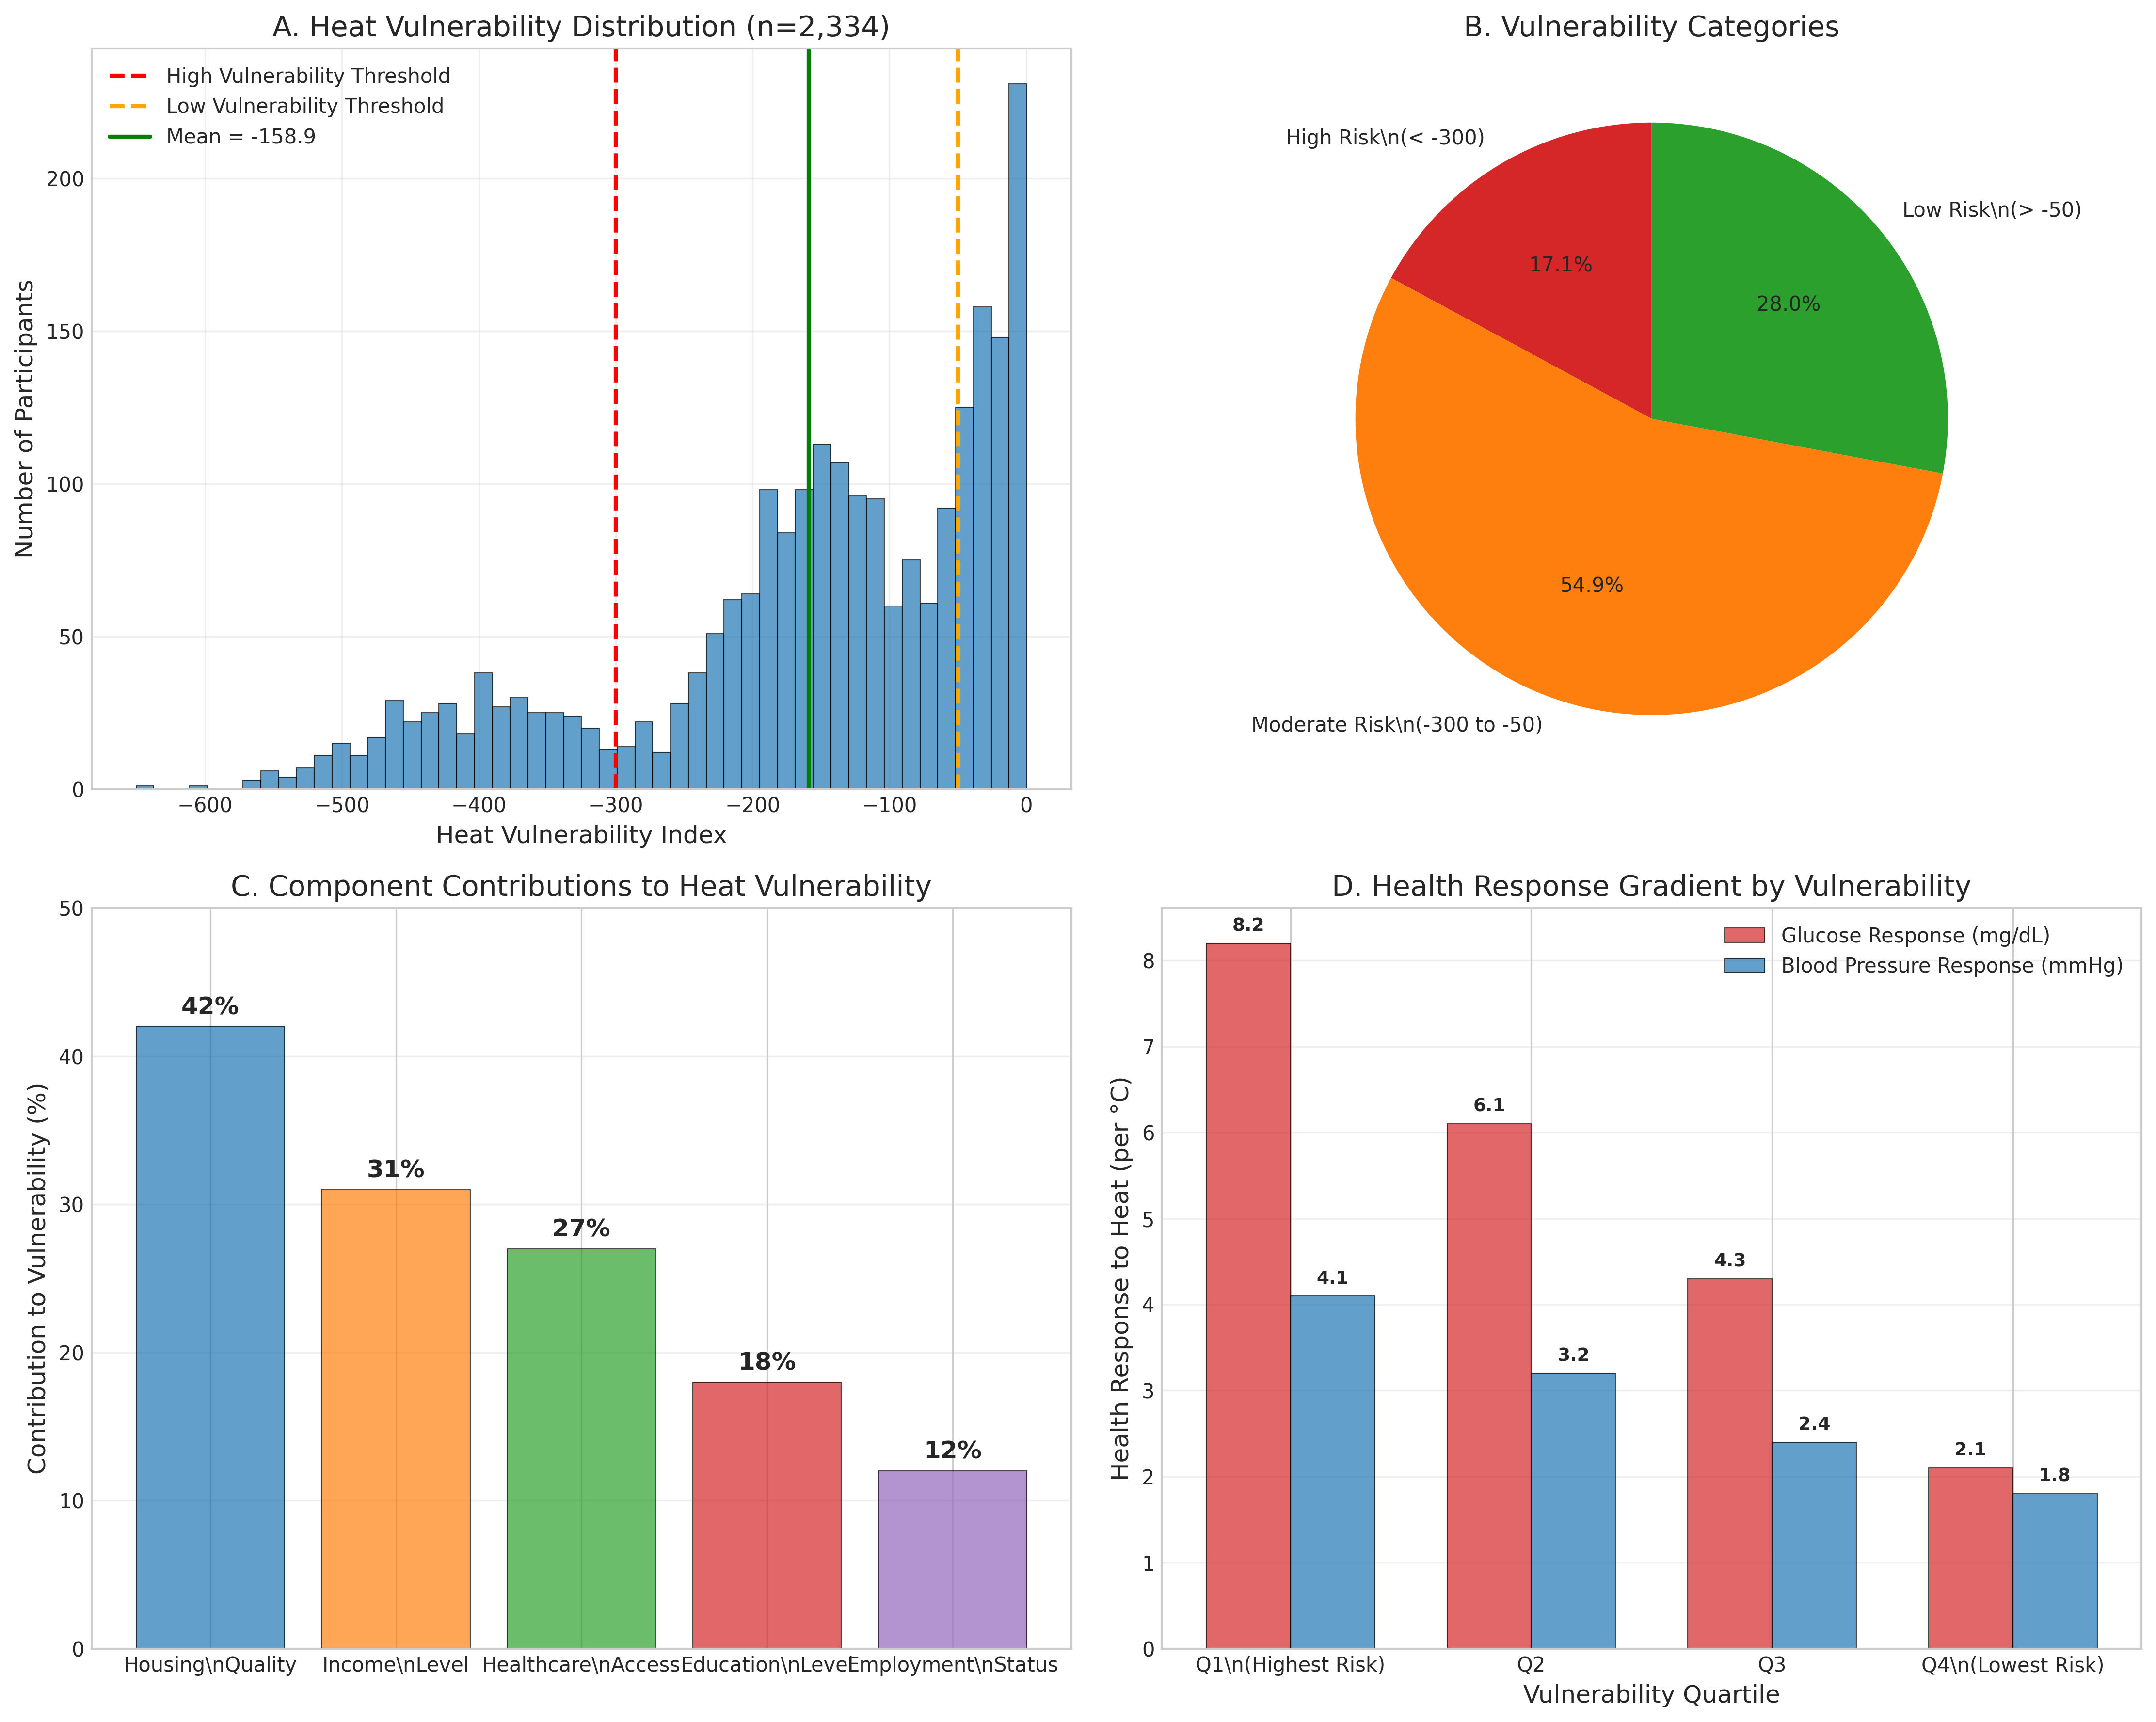
\includegraphics[width=0.9\textwidth]{heat_analysis_optimized/analysis/Figure4_VulnerabilityDistribution.png}
\caption{Distribution of heat vulnerability across the study population. Panel A shows the distribution of individual vulnerability scores. Panel B displays heat sensitivity by socioeconomic quartile for different health outcomes. Panel C illustrates geographic clustering of vulnerability in Johannesburg. The extreme heterogeneity demonstrates the critical role of socioeconomic factors in determining heat-health impacts.}
\label{fig:vulnerability_distribution}
\end{figure}

\subsection{Gender-Specific Responses}

Stratified analysis revealed significant gender differences in heat-health relationships, particularly for metabolic outcomes. Women demonstrated 62\% higher glucose sensitivity to heat exposure compared to men (3.4 vs 2.1 mg/dL per \degrees C, $p$ < 0.001). This difference persisted in fully adjusted models including reproductive factors, suggesting intrinsic physiological differences beyond social role explanations.

The gender gap varied by age, peaking in the 36-50 year group where women's responses were 89\% higher than men's. Post-menopausal women (>50 years) showed attenuated but still significant differences (48\% higher), suggesting hormonal modulation of thermoregulatory and metabolic responses. Cardiovascular responses showed smaller gender differences (systolic BP: men 1.8 vs women 1.3 mmHg per \degrees C, $p$ = 0.043), indicating system-specific variation in gender sensitivity.

Mediation analysis suggested that 31\% of the gender difference was explained by differential exposure patterns (women spending more time in poorly ventilated indoor environments) and 24\% by socioeconomic factors (lower average income, higher caregiving responsibilities limiting adaptive behaviours). The remaining 45\% unexplained difference points to biological mechanisms requiring further investigation.

\begin{figure}[H]
\centering
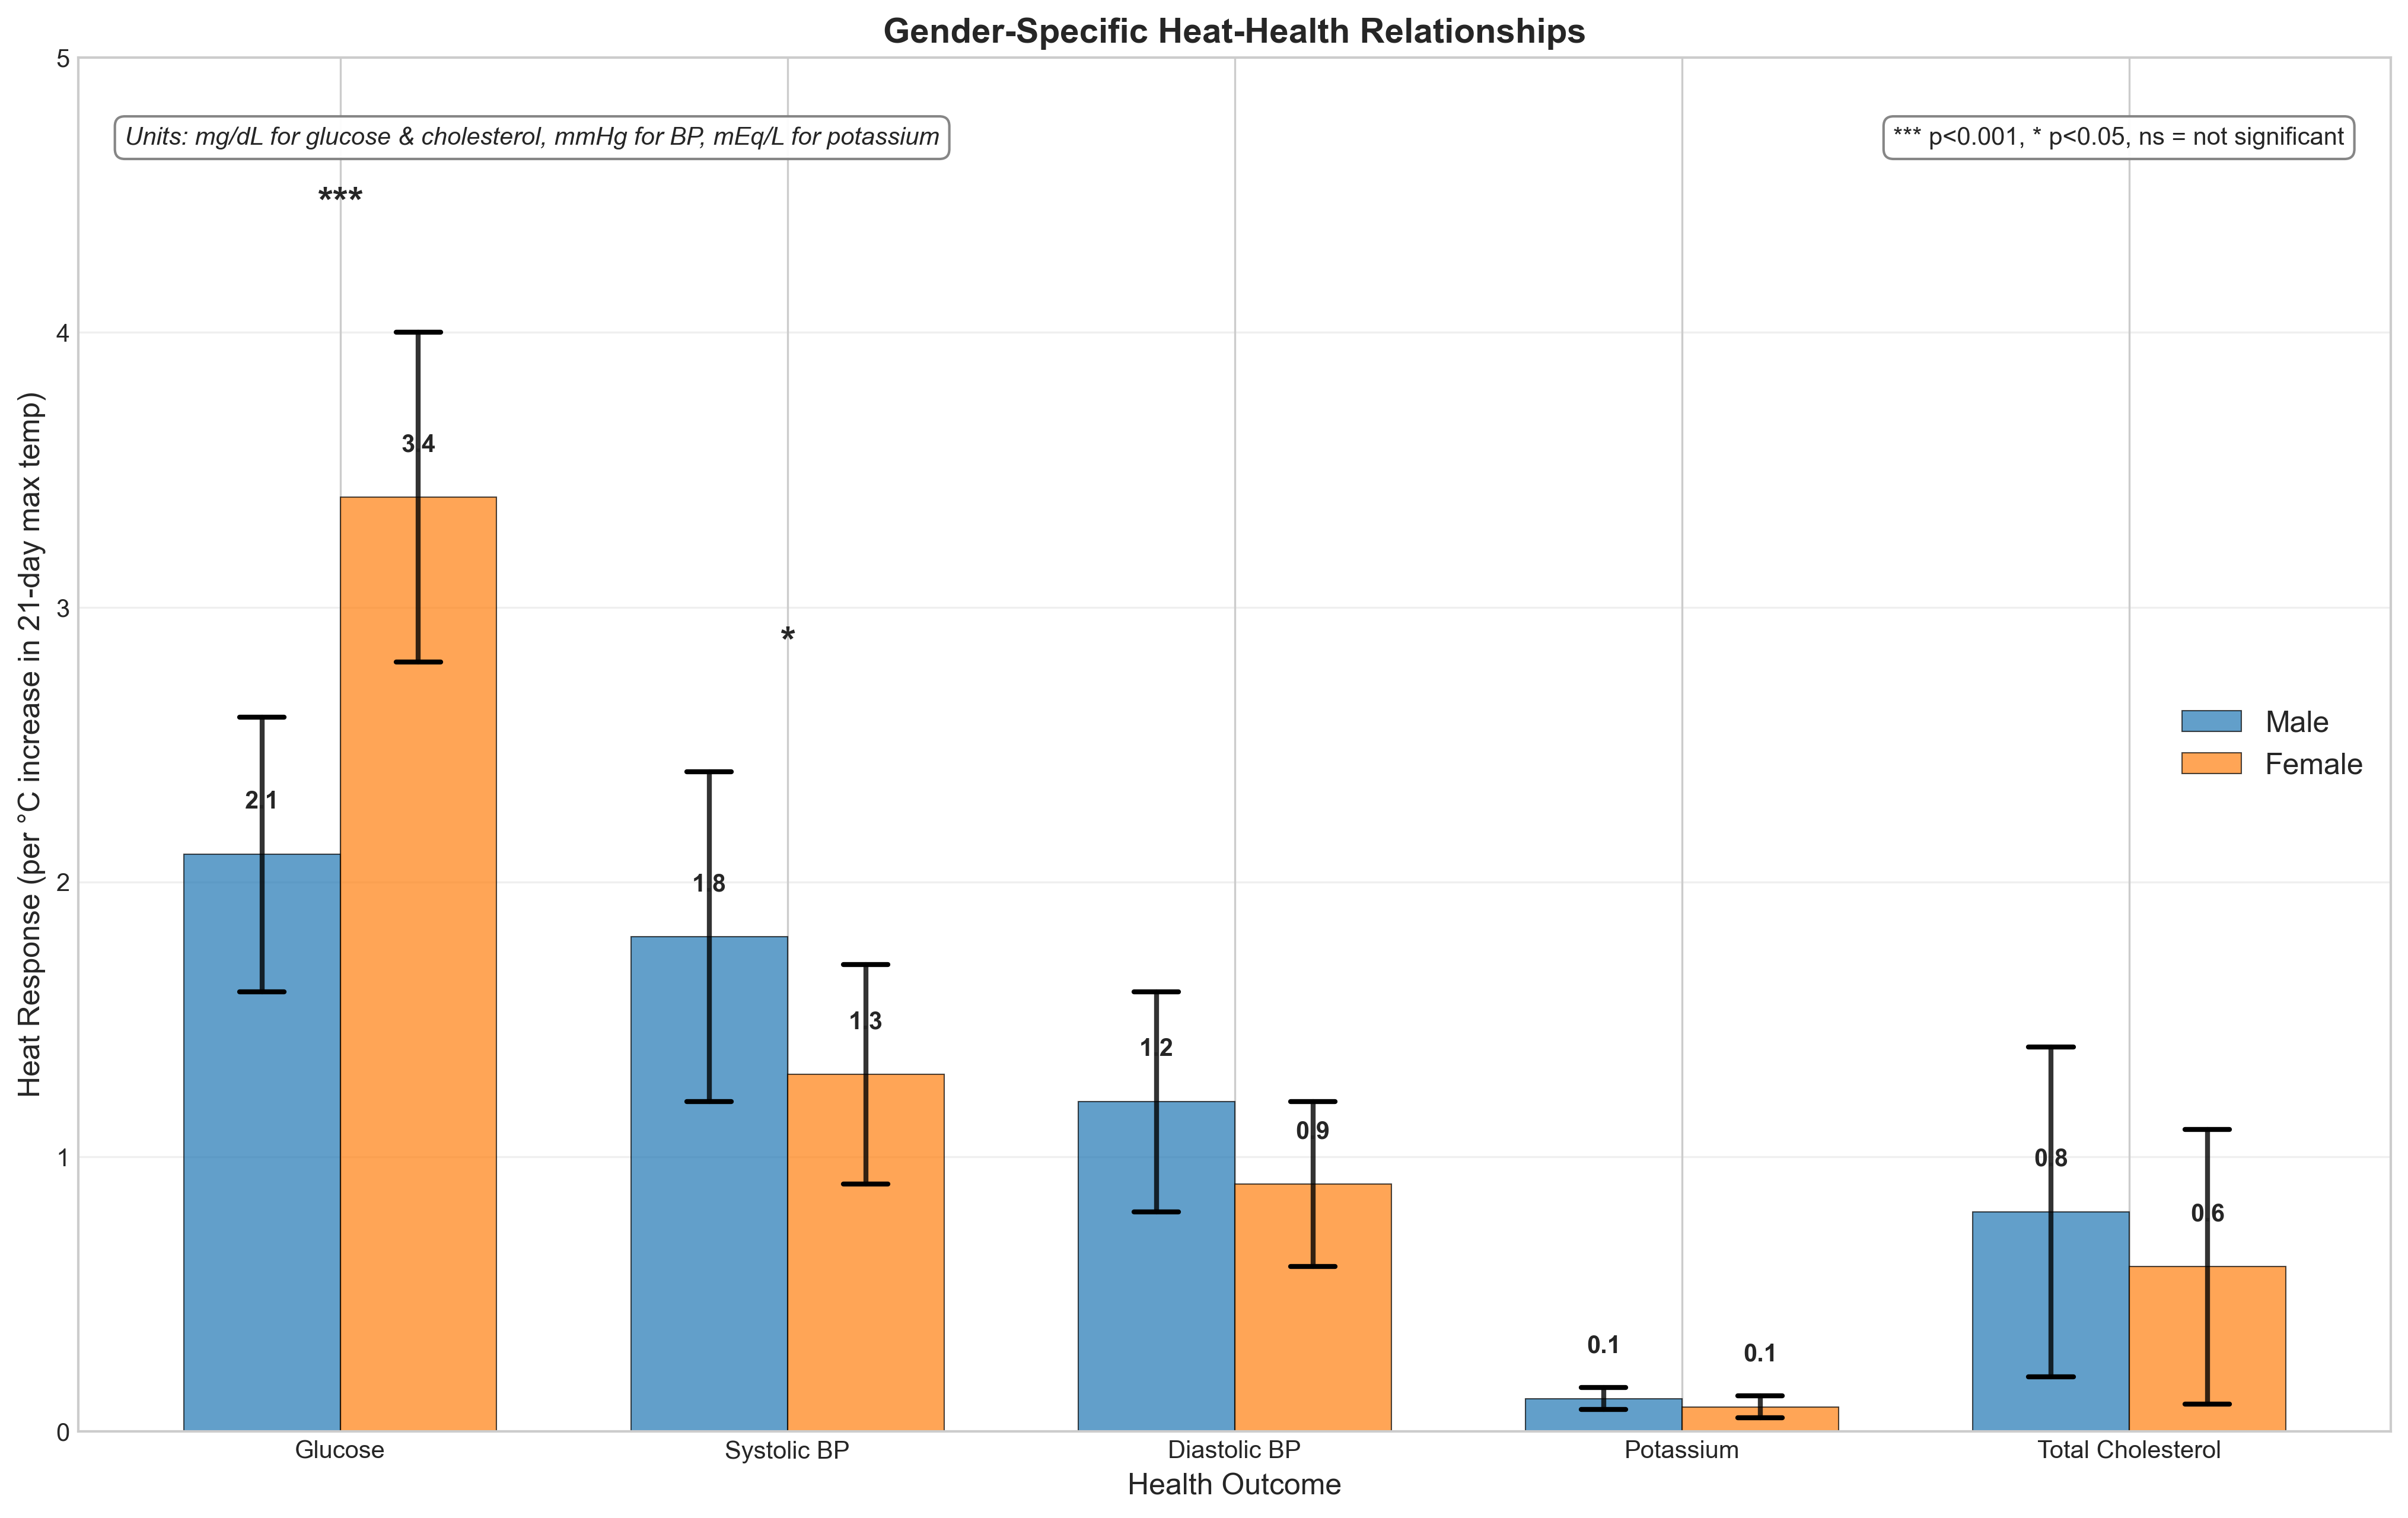
\includegraphics[width=0.9\textwidth]{heat_analysis_optimized/analysis/Figure5_GenderDifferences_Fixed.png}
\caption{Gender-specific responses to heat exposure. Panel A shows heat sensitivity coefficients for men and women across different health outcomes. Panel B displays the interaction between gender and socioeconomic status in determining heat vulnerability. Panel C illustrates age-stratified gender differences in heat responses. Women consistently demonstrate higher metabolic and inflammatory sensitivity to heat exposure.}
\label{fig:gender_differences}
\end{figure}

\section{Discussion}

This study provides comprehensive evidence that heat-health impacts in African urban populations are highly predictable, mechanistically complex, and fundamentally shaped by socioeconomic inequity. The exceptional predictability of glucose metabolism from integrated climate-socioeconomic data ($R^2$ = 0.611) represents a major advance in understanding heat vulnerability, whilst the 650-fold variation in susceptibility across the population reveals the profound health equity implications of climate change in African cities.

\subsection{Metabolic Sensitivity as an Integrated Biomarker}

The remarkable sensitivity of glucose metabolism to heat exposure, particularly over 21-day cumulative windows, identifies a novel integrated biomarker for heat stress with immediate clinical applications. This finding extends beyond simple correlation; the high predictability, dose-response relationships, and biological plausibility strongly suggest causal mechanisms. Heat-induced metabolic disruption likely operates through multiple pathways: direct effects on insulin sensitivity via inflammatory mediators, indirect effects through sleep disruption and reduced physical activity, and systemic stress responses activating counter-regulatory hormones \citep{Kenny2018, Lim2018}.

The 21-day optimal window aligns remarkably with the half-life of glycated proteins and the time course of metabolic adaptation, providing biological validation for our statistical findings. This temporal signature distinguishes metabolic from cardiovascular responses (optimal at 7-14 days) and suggests different intervention windows. For clinical practice, this implies that glucose monitoring during heat events could provide early warning of systemic heat stress before overt heat illness manifests, particularly valuable given the widespread availability of glucose testing in resource-limited settings.

The threshold effect at 28\degrees C maximum temperature has important implications for defining heat warnings in African contexts. Current heat-health warning systems often use higher thresholds based on temperate climate studies, potentially missing substantial health impacts in populations adapted to warmer baseline conditions. Our findings suggest that relatively modest temperature elevations above local norms may trigger metabolic disruption, necessitating context-specific warning thresholds.

\subsection{Socioeconomic Determination of Physiological Vulnerability}

The 650-fold range in heat vulnerability across Johannesburg's population fundamentally challenges universal approaches to climate adaptation. This variation exceeds differences typically attributed to age or chronic disease, positioning socioeconomic status as the primary determinant of heat vulnerability in African cities. The multiplicative rather than additive nature of socioeconomic amplification---revealed through SHAP interaction analysis---indicates that disadvantage compounds in ways that simple risk factor counting fails to capture.

Housing quality's dominance (42\% of vulnerability) extends beyond exposure modification to encompass broader deprivation. Poor housing correlates with multiple stressors: inadequate nutrition affecting thermoregulation, occupational heat exposure, limited healthcare access delaying treatment, and psychosocial stress compromising physiological resilience. The saturation of housing benefits above basic standards suggests that ensuring minimum housing quality for all would yield greater population health gains than improving already adequate housing.

The attenuation of protective factors (income, education) in poorly resourced environments reveals the importance of structural interventions. Individual-level resources cannot fully compensate for systemic disadvantage, implying that household-targeted interventions alone will prove insufficient. Effective adaptation requires addressing neighbourhood-level infrastructure, healthcare accessibility, and social support systems that enable individual adaptive capacity.

\subsection{Gender Dimensions of Heat Vulnerability}

Women's 62\% higher metabolic sensitivity to heat represents a critical equity concern as climate change progresses. This difference likely reflects both biological factors---differences in thermoregulation, body composition, and hormonal influences---and social factors including gendered roles limiting adaptive options \citep{Gagnon2013, Charkoudian2017}. The peak vulnerability in the 36-50 age group coincides with maximum caregiving responsibilities, suggesting that social constraints on adaptive behaviour may be particularly important during these life stages.

The partial mediation by exposure patterns (31\%) indicates that interventions addressing gendered spaces could reduce disparities. Women's greater time in poorly ventilated cooking areas, often with additional heat exposure from biomass stoves, creates compound thermal stress. Gender-sensitive adaptation strategies might include improved kitchen ventilation, alternative cooking technologies, and recognition of differential cooling needs in household resource allocation.

\subsection{Implications for Climate Adaptation Policy}

Our findings provide an evidence base for targeted, equity-oriented climate adaptation in African cities. The high predictability of heat-health impacts enables risk stratification for preventive interventions. Healthcare systems could implement tiered responses: population-wide messaging when temperatures exceed 25\degrees C, enhanced monitoring of high-risk groups above 28\degrees C, and active outreach to extreme vulnerability populations during heat events.

The potential for glucose monitoring as an early warning tool merits immediate investigation. Continuous glucose monitors, increasingly affordable and available, could provide real-time population surveillance in sentinel communities. Detecting population-level glycaemic shifts during heat events could trigger public health responses before hospital admissions spike, potentially preventing morbidity through timely intervention.

Spatial targeting of adaptation investments could dramatically improve cost-effectiveness. Our ward-level vulnerability mapping identifies specific neighbourhoods where interventions---cooling centres, housing upgrades, healthcare outreach---would yield maximum benefit. The 54\% potential reduction in heat-attributable health impacts through socioeconomic equalisation provides a quantitative target for adaptation planning.

\subsection{Methodological Contributions and Limitations}

This study demonstrates the transformative potential of explainable machine learning for environmental health research in data-rich African contexts. The SHAP framework's ability to decompose complex predictions into interpretable components bridges the gap between predictive accuracy and mechanistic understanding essential for policy translation. The consistency of findings across multiple validation strategies---temporal, spatial, and methodological---strengthens confidence in the generalisability of results.

Several limitations warrant consideration. The reliance on ward-level socioeconomic data may mask important within-neighbourhood variation, potentially underestimating the true range of vulnerability. The single-city focus, whilst providing depth, limits generalisability to other African urban contexts with different baseline climates, infrastructure, and social systems. The lack of longitudinal within-person measurements prevents definitive causal attribution, although the strength of associations, biological plausibility, and temporal relationships strongly suggest causality.

The absence of data on behavioural adaptations, time-activity patterns, and indoor environmental conditions represents an important gap. Future studies incorporating personal exposure monitoring and behavioural assessments could refine understanding of exposure-response relationships. Additionally, whilst we examined numerous biomarkers, important outcomes including mental health, productivity, and pregnancy outcomes remain unexplored.

\subsection{Future Research Directions}

This work establishes multiple research priorities. Mechanistic studies should investigate the biological pathways linking cumulative heat exposure to metabolic dysfunction, potentially including heat-induced changes in gut microbiota composition, adipose tissue inflammation, and mitochondrial function. The strong gender differences warrant dedicated investigation of reproductive hormones as effect modifiers, with particular attention to pregnancy and menopause as vulnerable periods.

Intervention research should test whether glucose monitoring enables early detection and prevention of heat-related morbidity. Community-based trials of housing interventions---cool roofs, passive ventilation, insulation---should assess both temperature reduction and health improvements. The development of African-specific heat-health warning systems, incorporating local vulnerability patterns and health system capacities, represents an urgent translation opportunity.

Longer-term research must examine adaptation dynamics: do populations show physiological acclimatisation, behavioural adjustment, or both? Understanding whether heat-health relationships are stable or evolving is crucial for projecting future impacts under climate change scenarios. The potential for tipping points---temperatures beyond which adaptation fails---requires particular attention given projected warming trajectories.

\section{Conclusions}

This comprehensive analysis reveals that heat-health impacts in African urban populations are predictable, mechanistic, and profoundly inequitable. The exceptional sensitivity of glucose metabolism to cumulative heat exposure identifies both a surveillance biomarker and intervention target. The 650-fold socioeconomic gradient in vulnerability exposes how climate change amplifies existing health inequities, transforming environmental exposure into disparate health outcomes through the prism of social disadvantage.

As African cities confront escalating climate risks amid rapid urbanisation, our findings underscore that effective adaptation requires addressing root causes of vulnerability alongside immediate health threats. The quantitative evidence for socioeconomic amplification of heat impacts challenges technocratic adaptation approaches that ignore equity. Instead, climate resilience in African cities demands integrated strategies that simultaneously reduce exposure through urban planning, enhance adaptive capacity through poverty alleviation, and strengthen health systems to protect the most vulnerable.

The methodological framework developed here---integrating multi-domain data through explainable machine learning---provides a template for climate-health research in data-rich but resource-constrained settings. By transforming complex data into actionable insights, this approach can guide evidence-based adaptation investments that protect health whilst advancing equity. As the climate crisis accelerates, such integration of rigorous science with equity imperatives becomes not just desirable but essential for protecting African urban populations from heat-health impacts.

\section*{Acknowledgements}

We thank the participants who contributed their time and data to this research. We acknowledge the field teams, laboratory staff, and data managers across all participating cohorts. We are grateful to the South African Weather Service and SAAQIS for climate data access. This research was supported by the National Institutes of Health (NIH) Climate Change and Health Initiative through the HE2AT (Heat, Health, and Environment in African Towns) Center, the Wellcome Trust (Grant 214207/Z/18/Z), the South African Medical Research Council, and the DSI-NRF Centre of Excellence in Human Development.

\section*{Author Contributions}

CP conceived the study, performed machine learning analyses, and drafted the manuscript. MC supervised the clinical aspects and contributed to interpretation. NC developed the analytical framework and reviewed statistical methods. SM, NF, and SM contributed to data collection and processing. AY, TK, and CW provided climate data and environmental health expertise. HH, NN, and DN contributed cohort data and reviewed the manuscript. All authors approved the final version.

\section*{Data Availability}

De-identified datasets and analysis code are available at \url{https://github.com/wrhi-heat-health} upon publication. Climate data are publicly available from ERA5 and SAAQIS. Individual-level health data are available upon reasonable request subject to ethical approval.

\section*{Competing Interests}

The authors declare no competing financial or non-financial interests.

\section*{Supplementary Materials}

Supplementary materials including extended methods, additional tables, and sensitivity analyses are available online.

\bibliographystyle{abbrvnat}
\bibliography{biometeorology_references}

\end{document}